
%%%%%%%%%%%%%%%%%%%%%%%%%%%%%%%%%%%%%%%%%%%%%%%%%%%%%%%%%%
\chapter{Conclusions and Future Work}
\label{chapter_conclusions_and_future_work}
%%%%%%%%%%%%%%%%%%%%%%%%%%%%%%%%%%%%%%%%%%%%%%%%%%%%%%%%%%

\section{Conclusions}

\newtext
{
We presented three deformation-driven packing methods.
FLOWPAK is a method to deform and pack long thin elements to follow a vector field.
RepulsionPak is a method that uses repulsion forces to pack and deform
elements that are represented as mass-spring systems.
AnimationPak is an extension of RepulsionPak that packs animated 2D elements,
each is an extruded 3D shape in a spacetime domain.
}

\newtext
{
Given a small size element library, 
we demonstrated that deformation-driven methods can create element compatibilities
and fill the container effectively.
Repeated elements give a sense of uniformity but deformation creates a sense of variety.
%As element compatibilities are increased, the negative space is more even.
}

\newtext
{
We discussed that the evenness of negative space is an indicator of the quality of a packing.
We measured the evenness using three statistical metrics:
spherical contact probabilities, histograms of distance transforms, and overlap functions.
}

\section{Future Work}

\newtext
{
We see many possibilities for further improvements to our methods and packing research.
}

\subsection{FLOWPAK}

%We see many possibilities for further improvements to our algorithm and
%future research on ornamental packing.  

\begin{itemize}

\item 
\newtext
{
\textbf{Element Threading:}
In FLOWPAK, an element must completely use up its streamline, 
causing a few elements to stretch too long.
We would like to combine multiple shorter elements
by threading them along streamlines, creating
a longer \textit{compound element} (Figure~\ref{thread_branch}a).
%This requires us to solve two potential challenges.
First, we need a way to connect the overlapping segments of the elements together
to create smooth and plausible transitions.
This possibly leads us to a deeper research topic:
how to develop a content-aware blending method on vector graphics patterns.
Second, we should carefully decide on the selection of elements we have to thread and
the number of elements we need. We would like to investigate a greedy approach
with backtracking~\cite{Kim2002}.
}

\item 
\newtext
{
\textbf{Element Branching:}
We also would like to support
branching structures to resemble floral ornaments (Figure~\ref{thread_branch}b).
We start with tracing a long streamline that follows the vector field,
and then generate shorter streamline branches,
which produce blobs that partly overlap the main blob.
Similarly, we also need to connect and blend element segments
at every intersection. 
We also should consider the semantics of the element shapes.
Not every part of an element can support branching; for example, a leaf
cannot be connected with twigs.
In another example, a stem or a trunk is an ideal segment where we can glue other elements.
}


\item \newtext{\textbf{High Curvature Streamlines:}}
FLOWPAK results do not have significant high-curvature streamlines like u-turns, 
since they could unpleasantly fold the decorative elements. This could be solved with a folding avoidance algorithm~\cite{Asente2010}.

\item \newtext{\textbf{Better Iterative Refinement:}}
The iterative refinement process uses a greedy approach, in which we 
iterate over all placed elements in a fixed order from smallest to largest.
We would like to investigate global optimizations
that could be applied to improve the overall composition in an 
order-independent way.  A natural first choice would be an approach based
on simulated annealing, although performance could become a more serious
issue in that case.
\newtext{
Another idea is to use RepulsionPak to refine the packing 
but we need to enforce a constraint on elements' spines to ensure they 
adhere to the vector field.
%but elements' spines still need to adhere to the vector field.
}

\item \newtext{\textbf{Automatic Fixed Element Creation:}}
We would like to explore the automatic creation and placement of 
the fixed elements, perhaps by discovering them as salient regions 
in source photographs, and extracting and vectorizing them.  This 
extraction must be carried out carefully, yielding enough fixed elements
to communicate a container clearly without disrupting the uniformity of
the design.

\end{itemize}

\begin{figure}
\centering
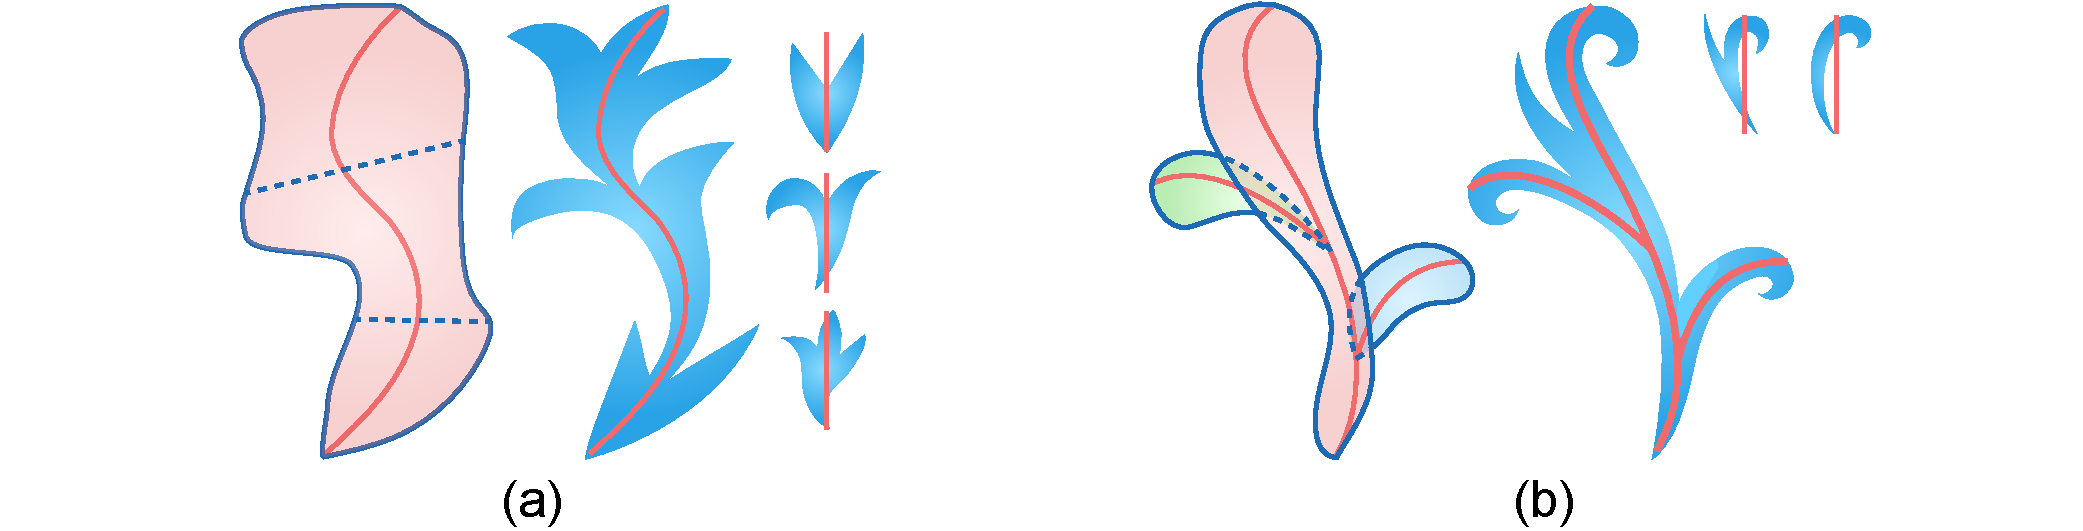
\includegraphics[width=1.0\textwidth]{figures/conclusions/thread_branch.pdf}
\caption[Element threading and branching]
{ \label{thread_branch} 
\newtext
{
(a) Thread multiple elements on a single streamline.
(b) Combine multiple streamlines to create branching.
}
}
\end{figure}

\subsection{RepulsionPak}

%We see many possibilities for further improvements to RepulsionPak
%and future research on element packings.

\begin{itemize}
\item 
\newtext{
	\newtext{\textbf{Improving the Numerical Integrator:}}
	We deliberately chose a simple 
	simulation model based on springs and forward Euler integration,
	because our main goal was to demonstrate the validity of a 
	deformation-driven approach, and not to contribute a new
	physical simulation method.}
	Contemporary research has yielded many more sophisticated 
	physical simulation methods, such as Position Based Dynamics~\cite{Muller2007}, 
	Projective Dynamics~\cite{Bouaziz2014}, and the Finite Element Method.
	No one method is obviously best suited to this problem, and
	we intend to experiment with several to investigate if any offers
	a suitable trade-off between performance and quality.

\item \newtext{\textbf{RepulsionPak for Fabrication:}} 
We would like to explore the use of RepulsionPak in a fabrication context.
      For example, our boundary compatibilities might be used to create a connected object.
      Alternatively, it would be interesting to 3D print the 
      negative space, which is already connected,
	  leaving holes that surround the element shapes.

\item \newtext{\textbf{Vector Graphics Warping:}}
Our barycentric warping method can
	introduce undesirable artifacts in highly deformed elements, as
	in the swallow tails in the left result of Figure~\ref{three_packings}.
	We would like to explore other methods for warping an element's
	geometry based on the correspondences between the triangles of its original
	mesh and the deformed meshes in the final packing, based for example on the
	work of Jacobson et al.~\cite{Jacobson2011} and Liu et al.~\cite{Liu2014}.


\item \newtext{\textbf{Interactive packings:}
  We would like to develop human-in-the-loop interactions, in
  which the user and the computer work together to create a desired
  composition.  Examples of recent work in this style include research
  by Zehnder et al.~\cite{Zehnder2016}, Gieseke et
  al.~\cite{Gieseke2017}, and Hsu et al.~\cite{Hsu2020}, which let the user directly place and manipulate
  elements while a composition is being created.
  It would also be interesting to display an interactive packing on a large touch screen,
  and let people to move elements around by touching and dragging gestures.}

\end{itemize}

\subsection{AnimationPak}

%We see an number of opportunities for improvements and extensions to
%AnimationPak:

\begin{itemize}
\item \newtext{\textbf{2D Vector Graphics Interpolation:}}
Because we use linear interpolation to \newtext{render} an element's shape
	between slices, we require elements not to undergo changes in 
	topology.  More sophisticated representations of vector shapes,
	such as that of Dalstein et al.~\cite{Dalstein2015}, could support
	interpolations between slices with complex topological changes.
	We would also need to synthesize a watertight envelope around the
	animating element in order to compute overlap and repulsion forces.

\item \newtext{\textbf{Dynamic Mesh Resolution:}}
We would like to improve the performance of the physical simulation.
	One option may be to increase the resolution of element meshes 
	progressively during simulation.  Early in the process, elements are
	small and distant from each other, so lower-resolution
	meshes may suffice for computing repulsion forces.

\item \newtext{\textbf{Continuous Collision Detection:}}
	Our discrete simulation can miss element overlaps that occur between
	slices.  A more robust continuous collision detection (CCD) algorithm
	such as that of Brochu et al.~\cite{Brochu2012}
	could help us find all collisions between
	the envelopes of spacetime elements.

\item \newtext{\textbf{Secondary Elements:}}
In RepulsionPak~\cite{Saputra2018}, an additional pass with
	small secondary elements had a significant positive effect on the
	distribution of negative space in the final packing.  It may be
	possible to identify stretches of unused spacetime that can be filled
	opportunistically with additional elements.  The challenge would be
	to locate tubes of empty space that run the full duration of the animation
	\newtext{and have sufficient diameters to accommodate added elements.}
	%always of sufficient diameter to accommodate an added element.

\item \newtext{\textbf{Animated Containers:}}
Like the spectral method~\cite{Dalal2006}, and unlike
	Animosaics~\cite{Smith2005}, AnimationPak can pack animated 
	elements into a static container.  We would like to extend
	our work to also handle animated containers. 
	\newtext
	{
	As demonstrated by the packing with a loose bird in Figure~\ref{fig_bib_entering_star},
	elements can vary their slice sizes to adapt to changes in container area.
	A more challenging solution is adding and removing elements,
	as this would certainly affect the initial element placement, which 
	would need to ensure that elements are placed fully inside the
	spacetime volume of the container.  		
	%It would be interesting to investigate whether we could adapt to changes in
	%container area		
	%It would be interesting to investigate whether we could adapt to changes in
	%container area by adding and removing elements. 
	%We are certain that it would not create undesirable element scaling as demonstrated 
	%by the packing in Figure~\ref{fig_bib_entering_star}.
	%However, this extension would certainly affect the initial element placement, which 
	%would need to ensure that elements are placed fully inside the
	%spacetime volume of the container.  
	}

\item \newtext{\textbf{Deformation-Driven 3D Packings:}}
AnimationPak implements forces and constraints geared towards 
	spacetime animation, but many of the same ideas could be adapted
	to develop a deformation-driven method for packing purely spatial
	3D objects into a 3D container.  We would like to evaluate the
	expressivity and visual quality of deformation-driven 3D packings 
	in comparison to other 3D packing techniques.

\item \newtext{\textbf{User Study with Artists:}}
There are many examples of static two-dimensional packings
	created by artists, which can serve as inspiration for an algorithm like RepulsionPak.  
	We were only able to find a single example of animated packing from The Simpsons (Figure~\ref{fig_animationpak_lisa_packing}). 
	We think its unpopularity is because it is difficult and time-consuming to create by hand.
	\newtext{Therefore,} we would like to engage with artists to understand the aesthetic value and limitations
	of AnimationPak.

\end{itemize}

\subsection{Packing Evaluation}

\begin{itemize}

\item \newtext{\textbf{Human Perception of the Evenness:}} We would like to conduct experiments that investigate the
  extent to which quantitative measurements of the evenness of negative
  space in a packing correlate with the human perception of a
  packing's quality.  In informal evaluations, some viewers found that
  the packing in Figure~\ref{balabolka_comparison}b, created with RepulsionPak,
  was packed more tightly than the artist's packing in
  Figure~\ref{balabolka_comparison}a, even though both have the same total
  amount of negative space.

%\item As with many research projects in non-photorealistic rendering, this
%work raises deep questions about the aesthetics of ornamental packings.
%What compositions are most appealing?  What is the most effective
%way to distribute negative space?  Some hand-drawn compositions insert additional small elements,
%like circles and squares, to break up large areas of negative space;
%an automated simulation of this process would be helpful.

\item \newtext{\textbf{Measuring Other Design Principles:}} We would like to develop additional metrics to evaluate
  how well an ornamental design fulfills other design principles.
  A measure of element deformation in a composition would permit 
  a comparison against future deformation-driven techniques.
  \newtext{In Chapter~\ref{chapter_flowpak}, we argue that visual flow and
  ``uniformity amidst variety'' are important to attractive packings.} 
  In another study, Wong et al.~\cite{Wong1998} describe basic design
  principles for decorative arts: repetition, balance, and conformation
  to geometric constraints.  The rigorous expression of aesthetic principles
  is a fascinating area for future research.

\item \newtext{\textbf{Different Offsetting for SCP:}}
Our validation metrics are all based on Minkowski sums or
  differences with discs, corresponding to a form of shape offsetting
  where corners become round.  The result of this rounding is visible in
  our graphs, for example in the gradual flattening of the SCP for
  the squares in Figure~\ref{hsr_viz}e.  It would be worthwhile to repeat
  these measurements using mitered offsetting, and to evaluate whether
  rounded or mitered offsetting is a closer match to human perceptual
  judgment of evenness.

\item \newtext{\textbf{Better Visualization for SCP:}}
When comparing calibrated packings, SCPs communicate 
  differences in the evenness of negative space, but the differences 
  between SCPs can be subtle.  In addition to distance histograms, 
  we would like to investigate other visualizations of this information
  that might amplify these differences to make evaluation easier.

\item \newtext{\textbf{Evaluating 2D Animated Packings:}}
All three metrics are only for evaluating 2D packings.
  While they extend naturally to three purely spatial
  dimensions, it is not clear whether they can be 
  adapted to the spacetime context.  
  We would like to investigate
  spatial statistics for the quality of animated packings created by AnimationPak that correlate
  with human perceptual judgments.

\end{itemize}



%\mynote{TODO:
%\begin{packeditems}
%\item Enlarge figures
%\item Remove 1-2 text rows on a page if figures are too big.
%\item Landscape pages in AnimationPak? 
%https://tex.stackexchange.com/questions/337/how-to-change-certain-pages-into-landscape-portrait-mode
%\item streamline $sl$ and slice $s$
%\item Conclusions are past tense
%\item Figures after texts.
%\item RepulsionPak related work: Shape deformation algorithms: ARAP, Bounded Biharmonics, etc.?
%\item reference abbreviated names
%\end{packeditems}
%}
